
\begin{multicols}{2}
\textit{Au cours de cette étude, la Terre est assimilée à une sphère $\Gamma$ de centre O et de rayon R.}

\medskip

\begin{enumerate}
\item \textbf{REPERAGE SUR LA SPHERE TERRESTRE}\\

Considérons un point M sur la surface terrestre,
distinct des pôles Nord et Sud.
On notera N et S les deux pôles.\\

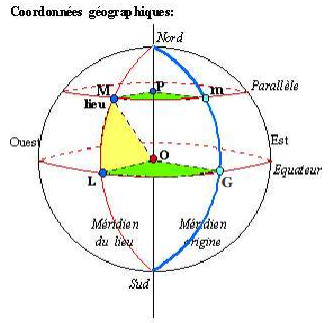
\includegraphics[scale=1]{RepE-coordonneesspheriques.png}


\begin{enumerate} 
\item \begin{enumerate}
	\item Définir le méridien Me de M.
	\item Définir le méridien de Greenwich.
		\end{enumerate}
\item \begin{enumerate}
	\item Définir le parallèle Pa de M.
	\item Définir l'équateur terrestre.
	\item Définir boréal et austral.
		\end{enumerate}
\item On note L l'intersection du méridien Me de M et de l'équateur.
	\begin{enumerate}
	\item Définir la latitude du point M.
	\item Quelle est la latitude d'un point de l'équateur ?
	\item Où sont situés les points de la surface terrestre qui ont même latitude que le point M ?
	\item Qu'appelle-t-on les tropiques du cancer et du capricorne ?
	\end{enumerate}
\item On note m le point d'intersection du parallèle Pa de M et du méridien de Greenwich.
	\begin{enumerate}
	\item Définir la longitude du point M.
	\item Quelle est la longitude d'un point du méridien de Greenwich ?
	\item Où sont situés les points de la surface terrestre qui ont même longitude que le point M ?
	\end{enumerate}
\item Définir les coordonnées géographiques de M.
\item Définir l'antipode du point M.
\item Rechercher :
	\begin{enumerate}
	\item Les coordonnées géographiques de Nouméa.
	\item Une ville du Brésil ayant même latitude que Nouméa.
	\item Une ville de Russie ayant même longitude que Nouméa.
	\item Le point du globe situé aux antipodes de Nouméa.

	\end{enumerate}
\end{enumerate}
\item \textbf{MESURE DE LA LATITUDE avec le gnomon}\\

Le jour de l'équinoxe à midi solaire en un point M de la Terre, le
soleil est à la verticale de l'équateur (au point l'équateur de même
longitude que M).
On considère le schéma en coupe de la Terre suivant le méridien Me
de M.\\

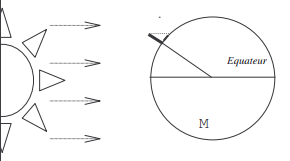
\includegraphics[scale=1]{RepE-schemacoupeterre.png}

\begin{enumerate}
\item En supposant que les rayons du soleil sont parallèles,
justifier que l'angle $\theta$ dans l'ombre du gnomon correspond à la
latitude de M.
\item On suppose que, dans les conditions précédentes, la tige du gnomon mesure 1 mètre
et que l'ombre projetée sur le sol mesure 80 cm, calculer au degré près l'angle $\theta$ dans
l'ombre du gnomon.

Sachant que vous êtes dans l'hémisphère nord, en déduire votre latitude.\\
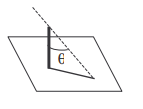
\includegraphics[scale=1]{RepE-angleteta.png}


\end{enumerate}
\item \textbf{MESURE DE LA LATTITUDE avec le sextant}\\

Le sextant a la forme d'un secteur angulaire de $60°$, soit un sixième de cercle, d'où le mot sextant.\\
Un sextant est composé de deux miroirs, un fixe (m) et un mobile (M). Lorsque l'alidade indique le $0°$ du limbe, les deux miroirs sont parallèles.

Le miroir fixe (m) est appelé miroir d'horizon. Sa moitié supérieure est transparente alors que sa moitié inférieure est réfléchissante.Lorsqu'on regarde dans la lunette de visée, la démarcation entre les deux moitiés du miroir (m) doit coïncider avec l'horizon. L'image directe et l'image réfléchie de l'horizon coïncident. Pour obtenir la hauteur $\alpha$ d'un astre, il suffit de déplacer le miroir mobile (M) jusqu'à ce que l'image de l'astre visé concorde avec la ligne d'horizon.\\

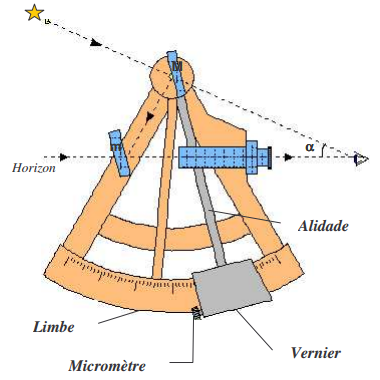
\includegraphics[scale=0.8]{RepE-sextant.png}


On va montrer que si, en visant toujours l'horizon, l'alidade pivote de l'angle
$2 \alpha$ alors le rayon incident
provient d'un astre à la hauteur $\alpha$.

\medskip

On considère le schéma en coupe du sextant donné ci-dessous:\\

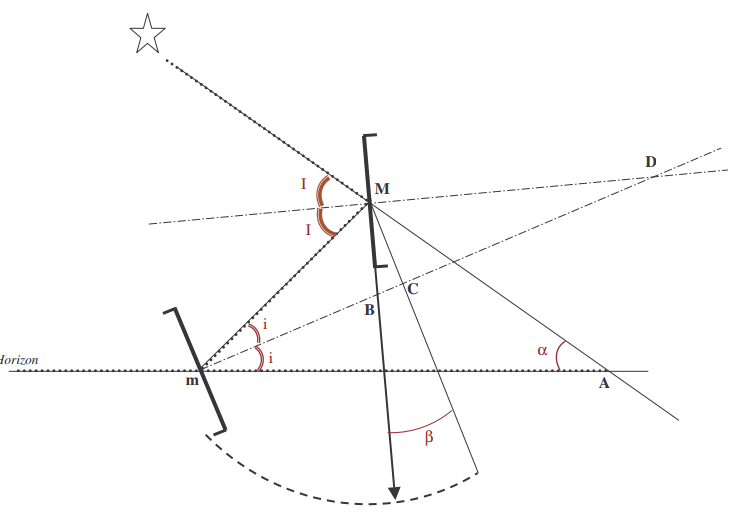
\includegraphics[scale=0.5]{RepE-schemacoupesextant.png} 

On note I et i les angles respectifs de réflexion sur les miroirs M et m.
\begin{enumerate}
\item \begin{enumerate}
	\item En utilisant le triangle mMA, montrer que $2i + \alpha + (180 – 2I) = 180$.
	\item En déduire l'expression de $\alpha$ en fonction de I et i.
	\end{enumerate}
\item \begin{enumerate}
	\item En utilisant le triangle MBC, exprimer la mesure de l'angle $\widehat{MBC}$ en fonction de $\beta$.
	\item En utilisant le triangle MBD, montrer que l'angle $\widehat{MDB}$ est égale à $\beta$.
	\item En utilisant le triangle mMD, montrer que $i + \beta + (180 – I) = 180$.
	\item En déduire l'expression de $\beta$ en fonction de I et i.
	\end{enumerate}
\item Conclure.

\item 
De fait, sur un sextant le limbe porte un secteur circulaire de $60°$ qui est gradué de $0°$ à $120°$. Ceci permet
d'obtenir, par lecture directe, la hauteur angulaire de l'astre.
On considère le schéma en coupe de la Terre suivant le méridien Me.
On note $\alpha$ la hauteur angulaire du soleil et $\delta$ la déclinaison du soleil. Expliquez.
\item Montrer que la latitude l du lieu est donnée par : $l = 90 + \delta – \alpha$ .
\item Justifier que le jour de l'équinoxe à midi solaire, la latitude du lieu est égale à $90 – \alpha$.
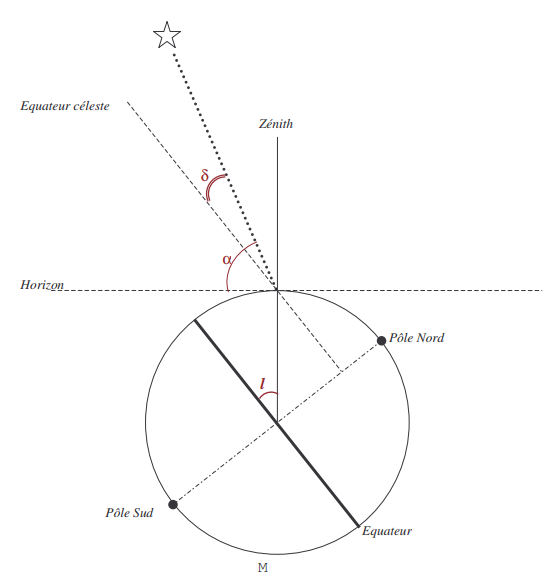
\includegraphics[scale=0.7]{RepE-schemacoupeme.png}

\end{enumerate}

\item \textbf{MESURE DE LA LONGITUDE}
\begin{enumerate}
\item De quel angle, en degrés, tourne la Terre en une minute.
\item On considère le schéma en coupe de la Terre suivant le parallèle P .\\

S'il est midi solaire au méridien de Greenwich, alors
que l'heure solaire est de 15 heures, quelle est la
longitude de M ?\\
 
La détermination de la longitude en navigation nécessitant la conservation de l'heure du méridien
d'origine, celle-ci n'a été, jusqu'au 19
ème
siècle, que très approximative au 18
ème
siècle, une horloge à
ressort était d'un imprécision allant jusqu'à une heure par jour.
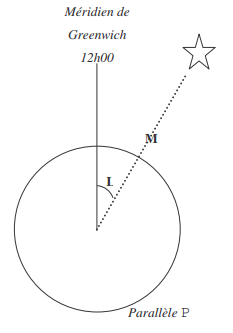
\includegraphics[scale=0.9]{RepE-schemacoupepa.png}

\end{enumerate}

\end{enumerate}
\end{multicols}



